\documentclass[12pt, a4, epsf] {article}
%==================================================
%Mypackages
\usepackage{epsf, amsmath, amssymb, graphicx, epsfig, amsthm}

\usepackage{subfigure} % For subfigures
\usepackage{setspace} 
\usepackage{fancyhdr} 
\usepackage{eurosym}  %To write a Euro symbol
\usepackage[euler]{textgreek}
\usepackage[english]{babel}
\usepackage[utf8]{inputenc}
\usepackage[colorlinks = true, urlcolor = blue, linkcolor = blue]{hyperref}
\usepackage{graphicx}
\usepackage{float}
\usepackage{bbm}
\usepackage{placeins}
\usepackage{pdfpages}
\usepackage{listings}
\usepackage{tikz}
\usetikzlibrary{graphs,graphs.standard}
\usetikzlibrary{shapes.geometric}
\usetikzlibrary{trees}
\usepackage{forest}
\usepackage{pdfpages}
\usepackage{algorithm} 
\usepackage{algpseudocode} 
%\usepackage[round]{natbib}


%Could change text height, width etc. 
\oddsidemargin 0mm
\evensidemargin 0mm
\textheight=24cm
\textwidth = 16cm
\topmargin= -1cm 

%Definition for theorems, definitions etc. for English texts
\theoremstyle{plain}
\newtheorem{theorem}{Theorem}[section]
\newtheorem{definition}[theorem]{Definition}
\theoremstyle{definition}
\newtheorem{example}[theorem]{Example}
\newtheorem{remark}[theorem]{Remark}


%==================================================
%My commands: Define your commands here:

\begin{document}
\begin{center}

{\Large Dummy Title\\}
By Dummies \\
27 JUN 2020
\end{center}

\section*{Abstract}
On April 24th, 2020, a researcher at MIT released a working paper finding that "The Subways Seeded the Massive Coronavirus Epidemic in New York City". While the analysis in the paper has been called into question, it remains true that the role of public transportation in the spread of COVID-19 is still unknown. In this paper, we introduce an agent-based model of the New York City subway and analyze how well it can predict the spread of COVID-19 through the boroughs of New York City.\\

Our findings that [insert findings here] should interest public health officials looking to make policy decisions about public transportation.

[Writer's Note: Of course, this is the ideal final result. We will focus on the early infection period and I give it a 50/50 that we even get to taking into account countermeasures and ridership losses. We will make a preliminary model, improve it, and see how far we can get.]

\section*{Competencies Briefing}
\textbf{Purpose: Brief others on competencies so we can discuss things\\}
\textbf{Transportation Networks\\}
\textit{specifically subways, the NYC subway. mapping, passenger flow\\}
\textbf{python, networkx, mesa\\}
\textit{we're working with these techs.\\}
\textit{Writer's Note: Obviously to be removed before submission\\}
\textit{This report was last pushed to OverLeaf on 30.05.2020. You will find our latest work at the link below:}
\url{https://github.com/cheung-ho-lum/NS_Epidemics_ABM_Approach/blob/master/Report/ABM_NYC_Subway.pdf}

\section*{Background}
\subsection*{Epidemics and COVID-19}
Coronavirus disease 2019 (COVID-19) is a disease caused by the SARS-CoV-2 coronavirus. Since being identified in December 2019, it has been labelled by the WHO as a pandemic, and spread around the world. Epidemics such as the 'coronavirus' have been a subject of research for centuries, and is of special interest to those working in public health. Recent waves of new research came in 2002 (SARS), 2009 (H1N1), and 2014 (Ebola). However, in these prior epidemics, researchers did not have access to as much data as we have currently. In recent years, the state of data science research tools have also greatly improved, allowing researchers to answer questions in novel ways, but following the scientific method. In this paper, we will try to respect the expertise of public health researchers, medical professionals, and the general public by being conservative when making conclusions.

\subsection*{The Seeding of COVID-19 in NYC}
\textit{Writer's note... ok. calling it seeding is overly negative about the original article\\}
In addition to general background knowledge about COVID-19, it would behoove the reader to know about the early spread of the disease in New York. Analysis of viral RNA in patients at the Mount Sinai Health System[\textbf{citation}] has lead researchers to conclude that the virus first came into the community through "multiple, independent but isolated introductions" from Europe and elsewhere in the USA. Below we have also given an approximate timeline of some of the most relevant events as of June 1st, 2020. We would also like to note that as forensic researchers begin examining the data, some significant new dates or corrections may arise:\\ 
\textit{Writer's Note: not working so hard on this because we might not need it.}\\
Feb 25 - Some guy came back from Iran\\
Mar 3 - First P2P spread\\
Mar 9 - 16 confirmed cases\\
Mar 9 (Approx.) - Metro ridership starts decreasing\\
Mar 16 - schools close. Measures already taken.\\
\textit{Writer's note: i.e. I'm uninterested, but depending on what research route we take (i.e. quarantine measures), this all may be relevant. }\\
Mar 18? - PAUSE government order to shelter in place\\
\subsection*{Epidemic Modeling}
\textit{Blah blah blah. I would like to briefly acknowledge the superiority of statistical modeling for the purpose of forecasting.}
\subsection*{SEIR Model}
[Some explanation of SEIR goes here]\\
\textit{Writer's note: I think SEIR is not great for covid. But it's somewhat useful for modeling interventions. Also the fact that poop has already hit the fan when you detect patient zero}
\subsection*{Newer Compartmental Models}
\textit{Writer's note: We're looking into more advanced models (see bibliography). The key additions are 'super-spreaders' and 'asymptomatic'. At the end of the day, we just need pure mathematically modeling to provide some parameters for how agents should behave.} 
\subsection*{Epidemics on Networks}
\subsection*{Agent Based Models}
It's just a tool. like any model. Simulating agents in an environment. Key parameters are agent, model, and environment parameters. For example, we have the following list thus far:\\
\begin{verbatim}
	(Agent)STATUS_SUSCEPTIBLE = 'Susceptible'
	(Agent)STATUS_EXPOSED = 'Exposed'
	(Agent)STATUS_INFECTED = 'Infected'
	(Agent)STATUS_INFECTED_ASYMPTOMATIC = 'Asymptomatic'
	(Agent)STATUS_RECOVERED = 'Recovered'
	(Agent)TIME_TO_RECOVER = 10
	(Agent)TIME_TO_INFECTION = 3
	(Model)RUN_SPAN = 60
	(Model)TOTAL_POPULATION = 50000
\end{verbatim}
The environment is new york subway mapped as a network.\\ 
All of this is still being discussed.\\
\subsection*{Urban Transportation Networks and Epidemics}
\subsection*{Subways and subway nomenclature}
This guy is indispensable for figuring out how to parse some of this data:\\
\url{https://en.wikipedia.org/wiki/New_York_City_Subway_nomenclature}\\
\textbf{The key is lines and routes}\\
\section*{Methodology}
\subsection*{MESA(Or our ABM)}
\textit{Writer's note: I'm a bit too lazy to learn tikz-uml. I'll just make a regular uml and... screenshot it\\}
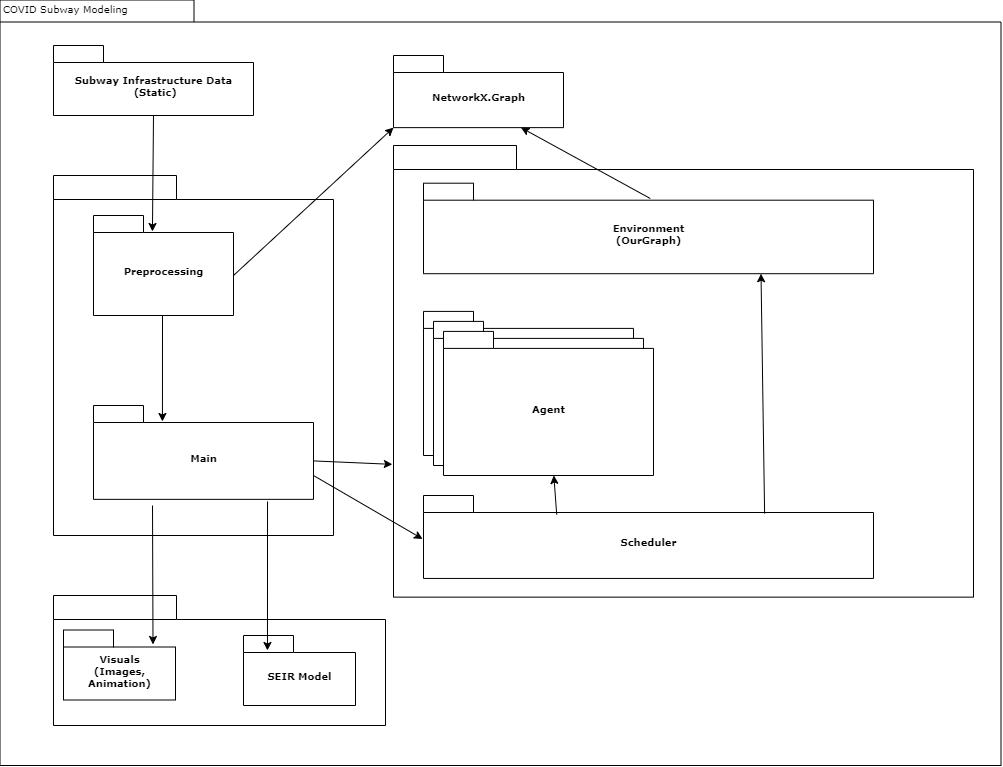
\includegraphics[width = 1.0\textwidth]{Scratch_Visuals/covid_subway.png}
\subsection*{NetworkX}
\subsection*{MTA Station Data}
\textbf{Station, Complex, Line, Route\\}
\textit{station 167... doubled\\}
\textit{making edges. GTFS Data... no we do it ourselves\\}
\subsection*{MTA Turnstile Data}
\textit{discuss format. every 4 hours, every machine. aggregation.\\}
\section*{Results}
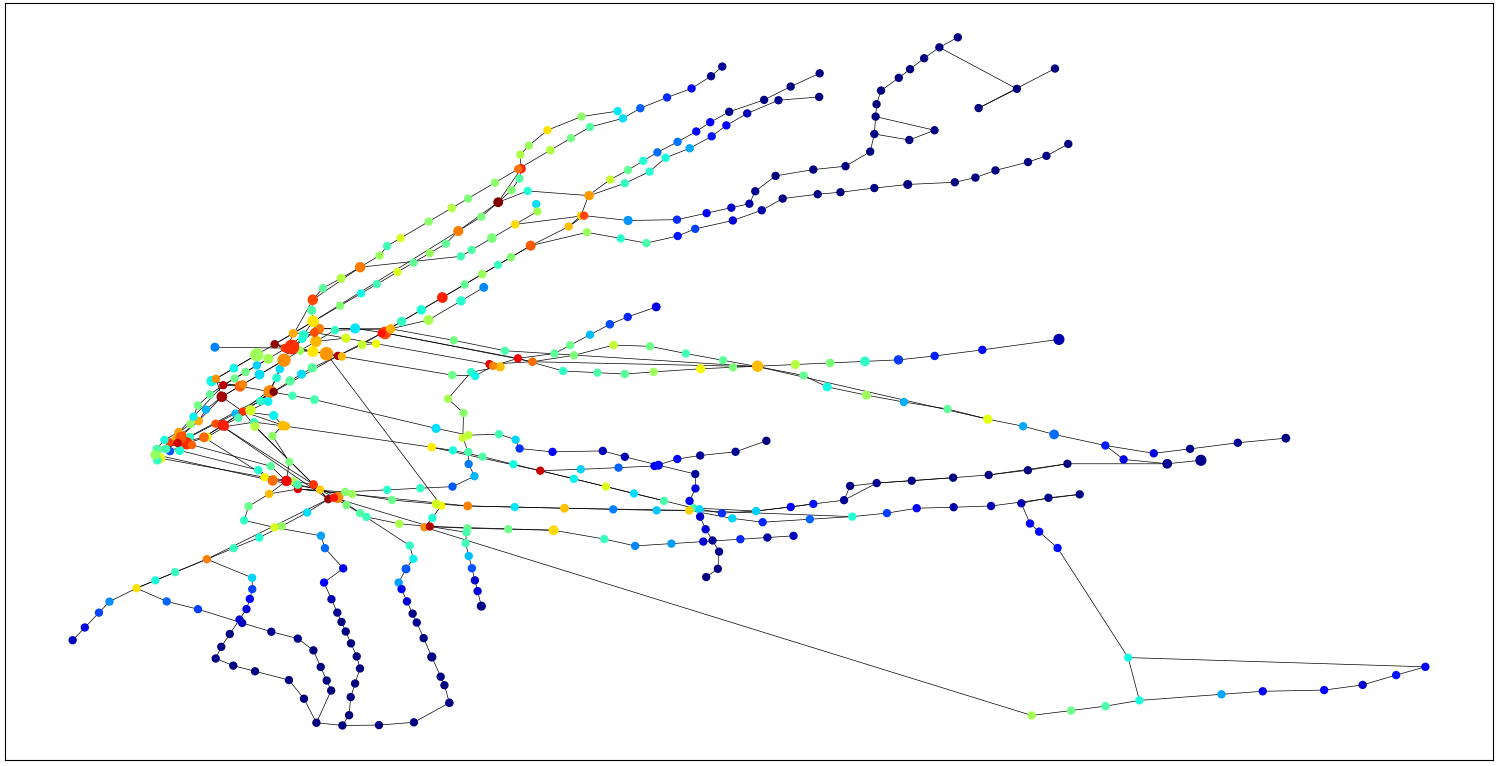
\includegraphics[width = 1.0\textwidth]{Scratch_Visuals/Preliminary_Modeling.png}
\section*{Conclusion}
\textbf{\textit{Writer's Note: All Models are Wrong, Some are Useful}}
\nocite{*}
\bibliography{bib_file}{}
\bibliographystyle{plain}

\end{document}
